\mathchardef\period=\mathcode`.
\documentclass[a4paper]{article}
\usepackage[top=1.45cm, bottom=1cm, left=1cm, right=1cm]{geometry}

\usepackage{parskip} % Package to tweak paragraph skipping
\usepackage{tikz} % Package for drawing
\usepackage{tkz-euclide}
\usepackage{siunitx}
\usepackage{wrapfig}
\usepackage{graphicx}
\usepackage{array}
\usepackage{changepage}

\usepackage{pgfplots}
\usetikzlibrary{fit,positioning}
\usetikzlibrary{arrows.meta}
\usetikzlibrary{patterns,patterns.meta}
\usetikzlibrary{calc,intersections}
\usetikzlibrary{angles, quotes}
\usetikzlibrary{shapes}
\usetikzlibrary{intersections,pgfplots.fillbetween}
\usepackage[inline]{enumitem}
\usepackage{amsmath,amssymb}
\usepackage{tasks}
\usepackage{amsmath}
\usepackage{hyperref}
\usepackage[main=lithuanian, german, shorthands=off]{babel}
\usepackage{tgpagella}
\usepackage[L7x,T1]{fontenc}
\usepackage[utf8]{inputenc}
\usepackage{enumitem}
\usepackage{booktabs} % For better looking tables
\usepackage{venndiagram}
\usepackage{subfig}
\usepackage{multirow}
\usepackage{tabularray}
\usepackage{lipsum}
\usepackage{fancyhdr}

\usepackage{blindtext}
\usepackage{adjustbox}
\AfterEndEnvironment{wrapfigure}{\setlength{\intextsep}{0mm}}

\usepackage{icomma}

% Header | Footer 
\fancyhf{} % clear all header and footer fields
\fancyhead[R]{ Trikampio panašumo požymiai | kontrolinis darbas }
\fancyfoot[R]{ Trikampio panašumo požymiai | kontrolinis darbas }
\setlength{\headheight}{0.5pt} % Adjust the head height
\renewcommand{\headrulewidth}{0.4pt} % Line under the header
\renewcommand{\footrulewidth}{0.4pt} % Line above the footer
% Header | Footer 

\newcommand{\germanqq}[1]{{\selectlanguage{german}\glqq#1\grqq\selectlanguage{english}}}

\DeclareMathOperator{\tg}{tg}
\newcommand{\tgx}{\tg x}

\DeclareMathOperator{\arctg}{arctg}
\newcommand{\arctgx}{\arctg x}

\makeatletter
\newcommand*{\rom}[1]{\expandafter\@slowromancap\romannumeral #1@}
\makeatother

\title{Trikampio panašumo požymiai | kontrolinis darbas }
\author{Vilius Paliokas}
\date{2024/01/17}

\setlist{after=\vspace{\baselineskip}}

% Title spacing
\usepackage{titlesec}
\titlespacing*{\subsection}{0pt}{.75ex}{0.75ex}

% ------------------------ 

\begin{document}
\thispagestyle{fancy}

\subsection*{1 variantas}

\begin{minipage}{0.5\textwidth}
      \begin{enumerate}
            \setcounter{enumi}{0} % This continues the numbering from the previous enumerate
            \item Remdamiesi brėžinyje pateiktais duomenimis:
                  \begin{tasks}[item-format={\normalfont}, after-item-skip=2mm](1)
                        \task Įrodykite, kad trikampiai $ABC$ ir $AED$ panašūs;
                        \task Raskite atkarpos $DE$ ilgį;
                        \task Trikampio $ADE$ plotą.
                  \end{tasks}
      \end{enumerate}

      \begin{center}
            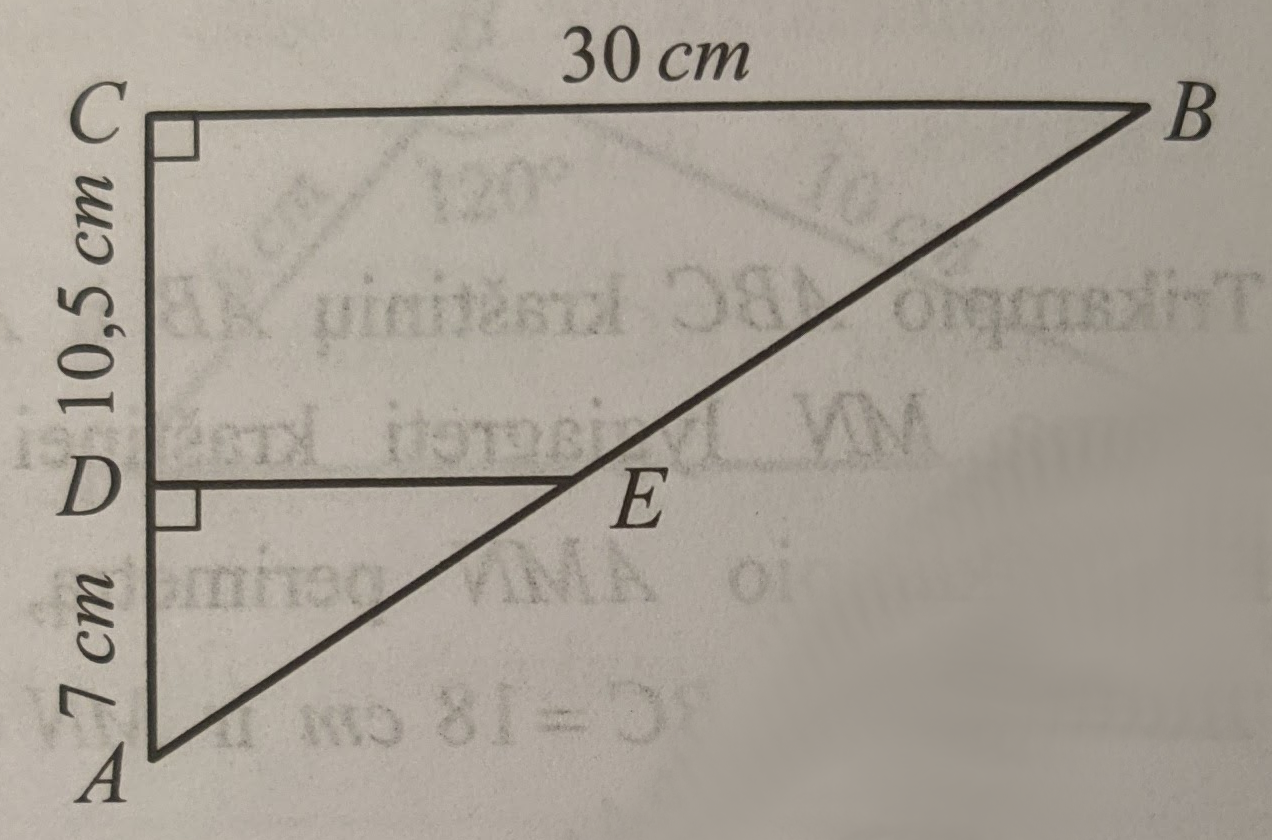
\includegraphics[scale=0.5]{images/triangle_1.png}
      \end{center}

\end{minipage}
\begin{minipage}{0.5\textwidth}
      \begin{enumerate}
            \setcounter{enumi}{1} % This continues the numbering from the previous enumerate
            \item Remdamiesi brėžinyje pateiktais duomenimis, įrodę, kad pateikti trikampiai
                  panašūs, apskaičiuokite trikampio $PRS$ kraštinės $PS$ ilgį.
      \end{enumerate}
      \begin{center}
            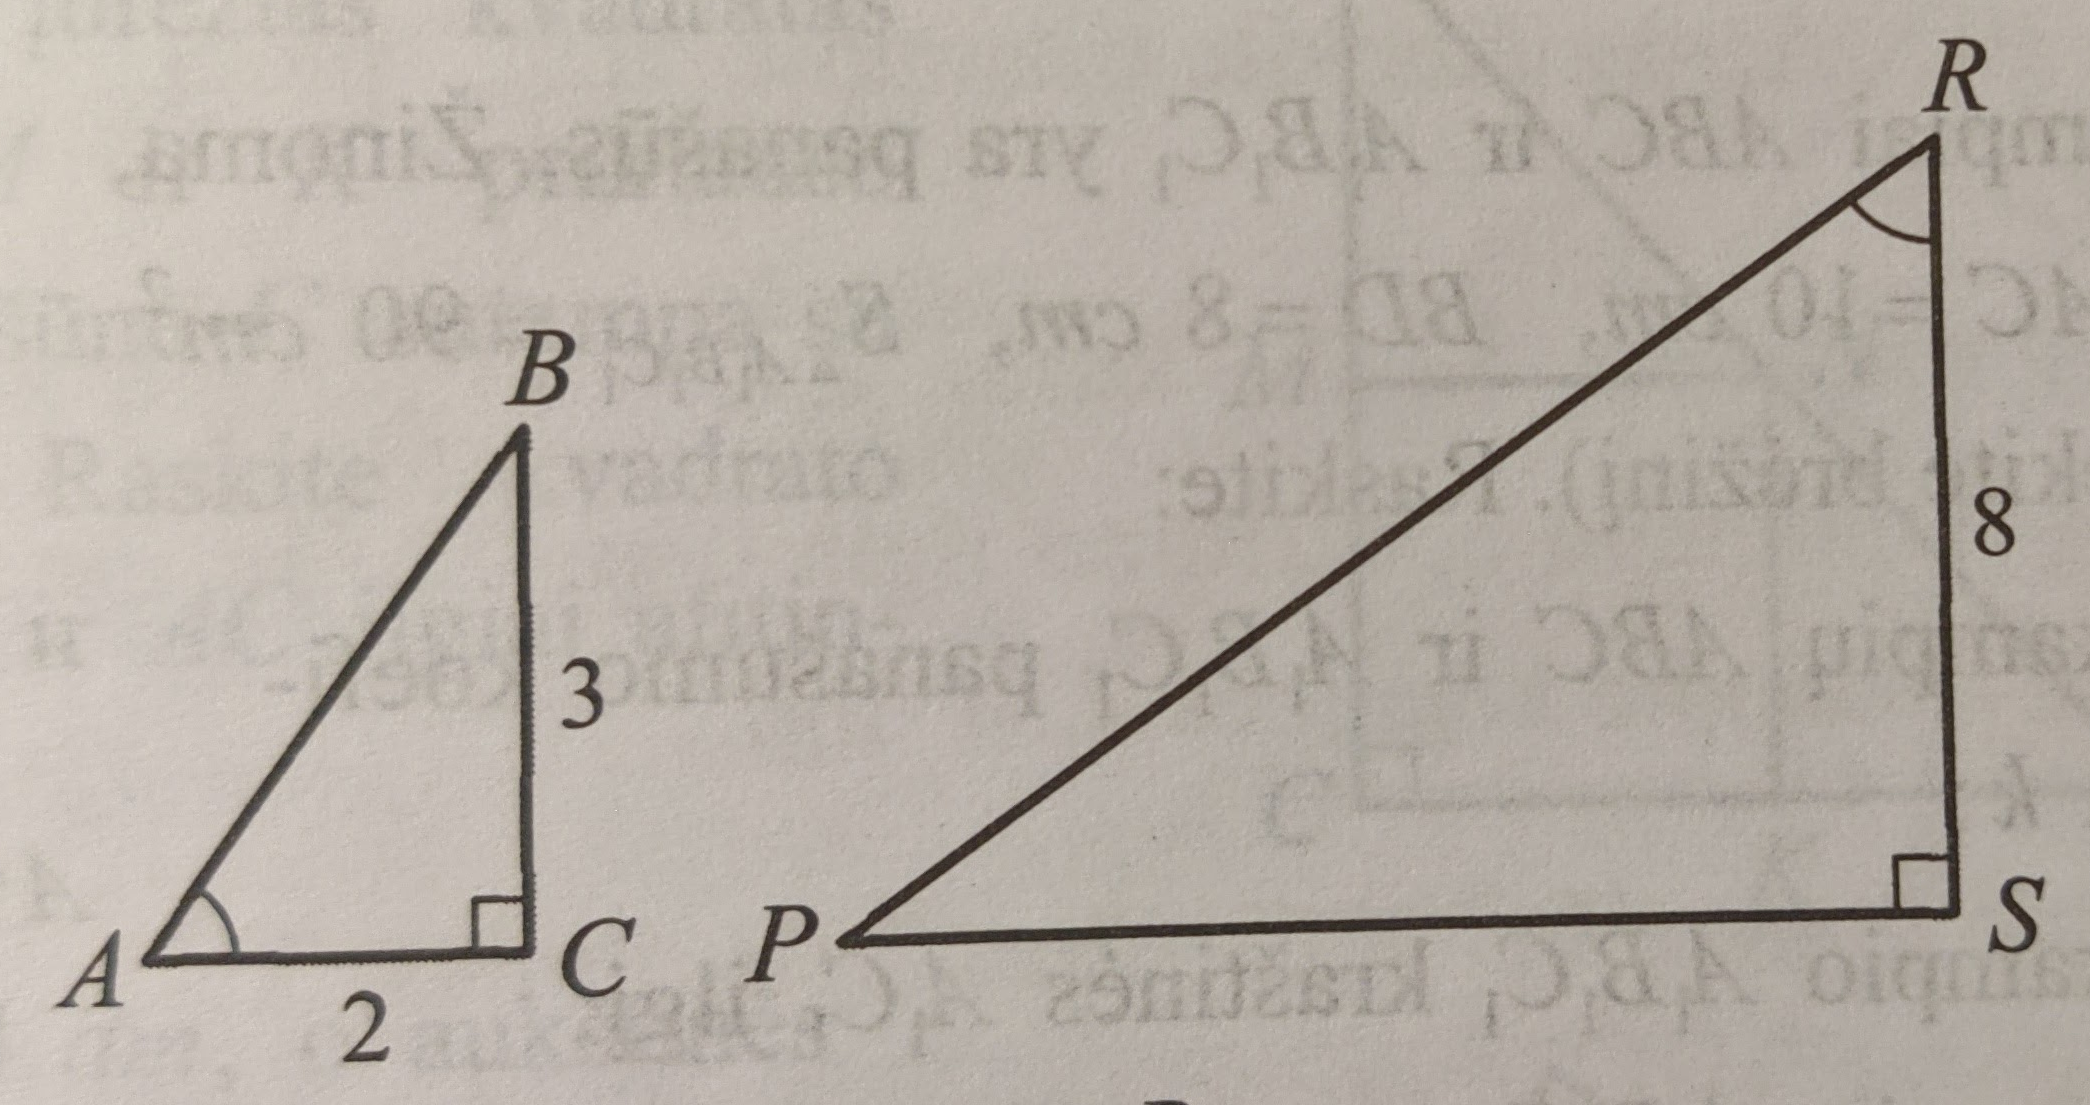
\includegraphics[scale=0.5]{images/triangle_2.png}
      \end{center}
\end{minipage}

\begin{enumerate}
      \setcounter{enumi}{2} % This continues the numbering from the previous enumerate
      \item Trikampiai $ABC$ ir $A_1B_1C_1$ yra panašūs. Žinoma, kad $AB=32 \; cm$,
            $A_1B_1=6,4 \; cm$, $S_{\triangle ABC}=64 \; cm^2$.
            \begin{tasks}[item-format={\normalfont}, after-item-skip=2mm](2)
                  \task Apskaičiuokite trikampio $A_1B_1C_1$ plotą;
                  \task Apskaičiuokite trikampių $A_1B_1C_1$ ir $ABC$ perimetrų santykį.
            \end{tasks}
\end{enumerate}

\subsection*{1 variantas}

\begin{minipage}{0.5\textwidth}
      \begin{enumerate}
            \setcounter{enumi}{0} % This continues the numbering from the previous enumerate
            \item Remdamiesi brėžinyje pateiktais duomenimis:
                  \begin{tasks}[item-format={\normalfont}, after-item-skip=2mm](1)
                        \task Įrodykite, kad trikampiai $ABC$ ir $AED$ panašūs;
                        \task Raskite atkarpos $DE$ ilgį;
                        \task Trikampio $ADE$ plotą.
                  \end{tasks}
      \end{enumerate}

      \begin{center}
            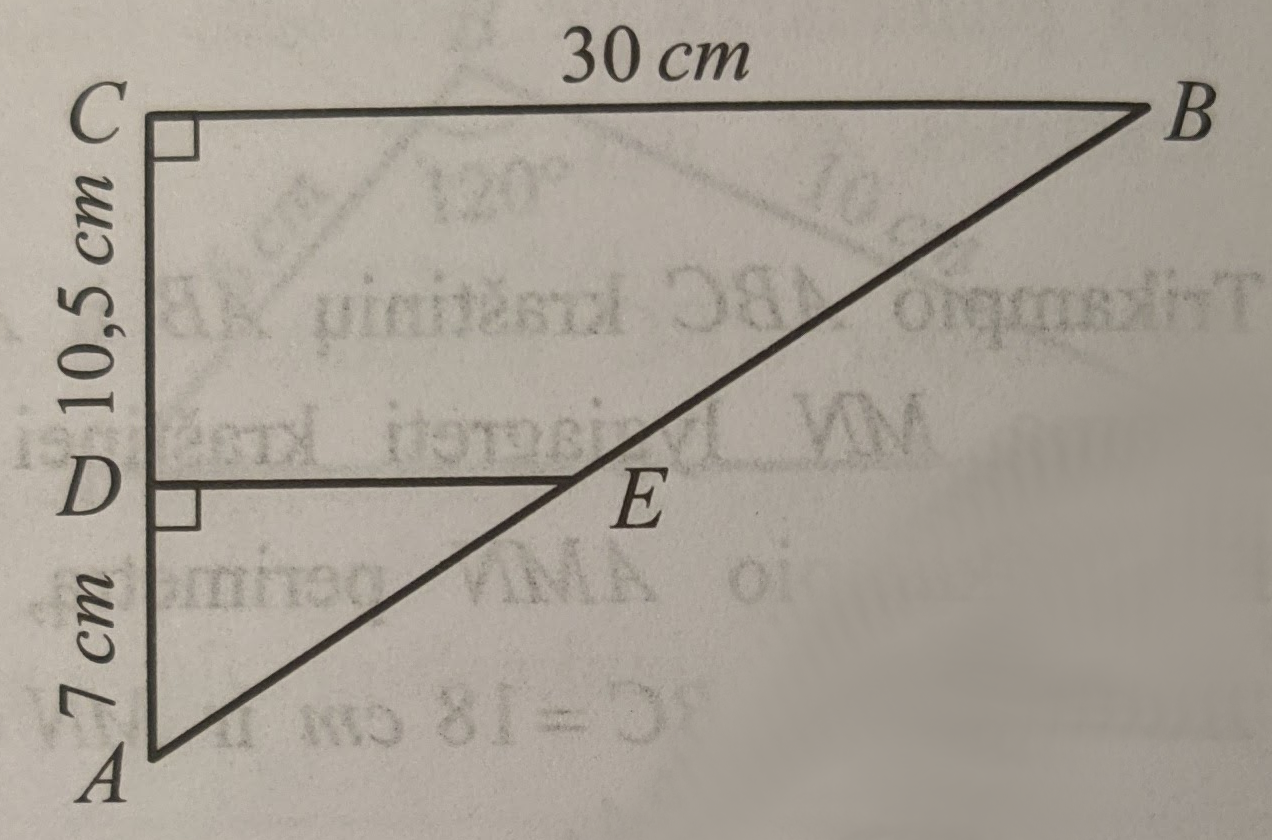
\includegraphics[scale=0.5]{images/triangle_1.png}
      \end{center}

\end{minipage}
\begin{minipage}{0.5\textwidth}
      \begin{enumerate}
            \setcounter{enumi}{1} % This continues the numbering from the previous enumerate
            \item Remdamiesi brėžinyje pateiktais duomenimis, įrodę, kad pateikti trikampiai
                  panašūs, apskaičiuokite trikampio $PRS$ kraštinės $PS$ ilgį.
      \end{enumerate}
      \begin{center}
            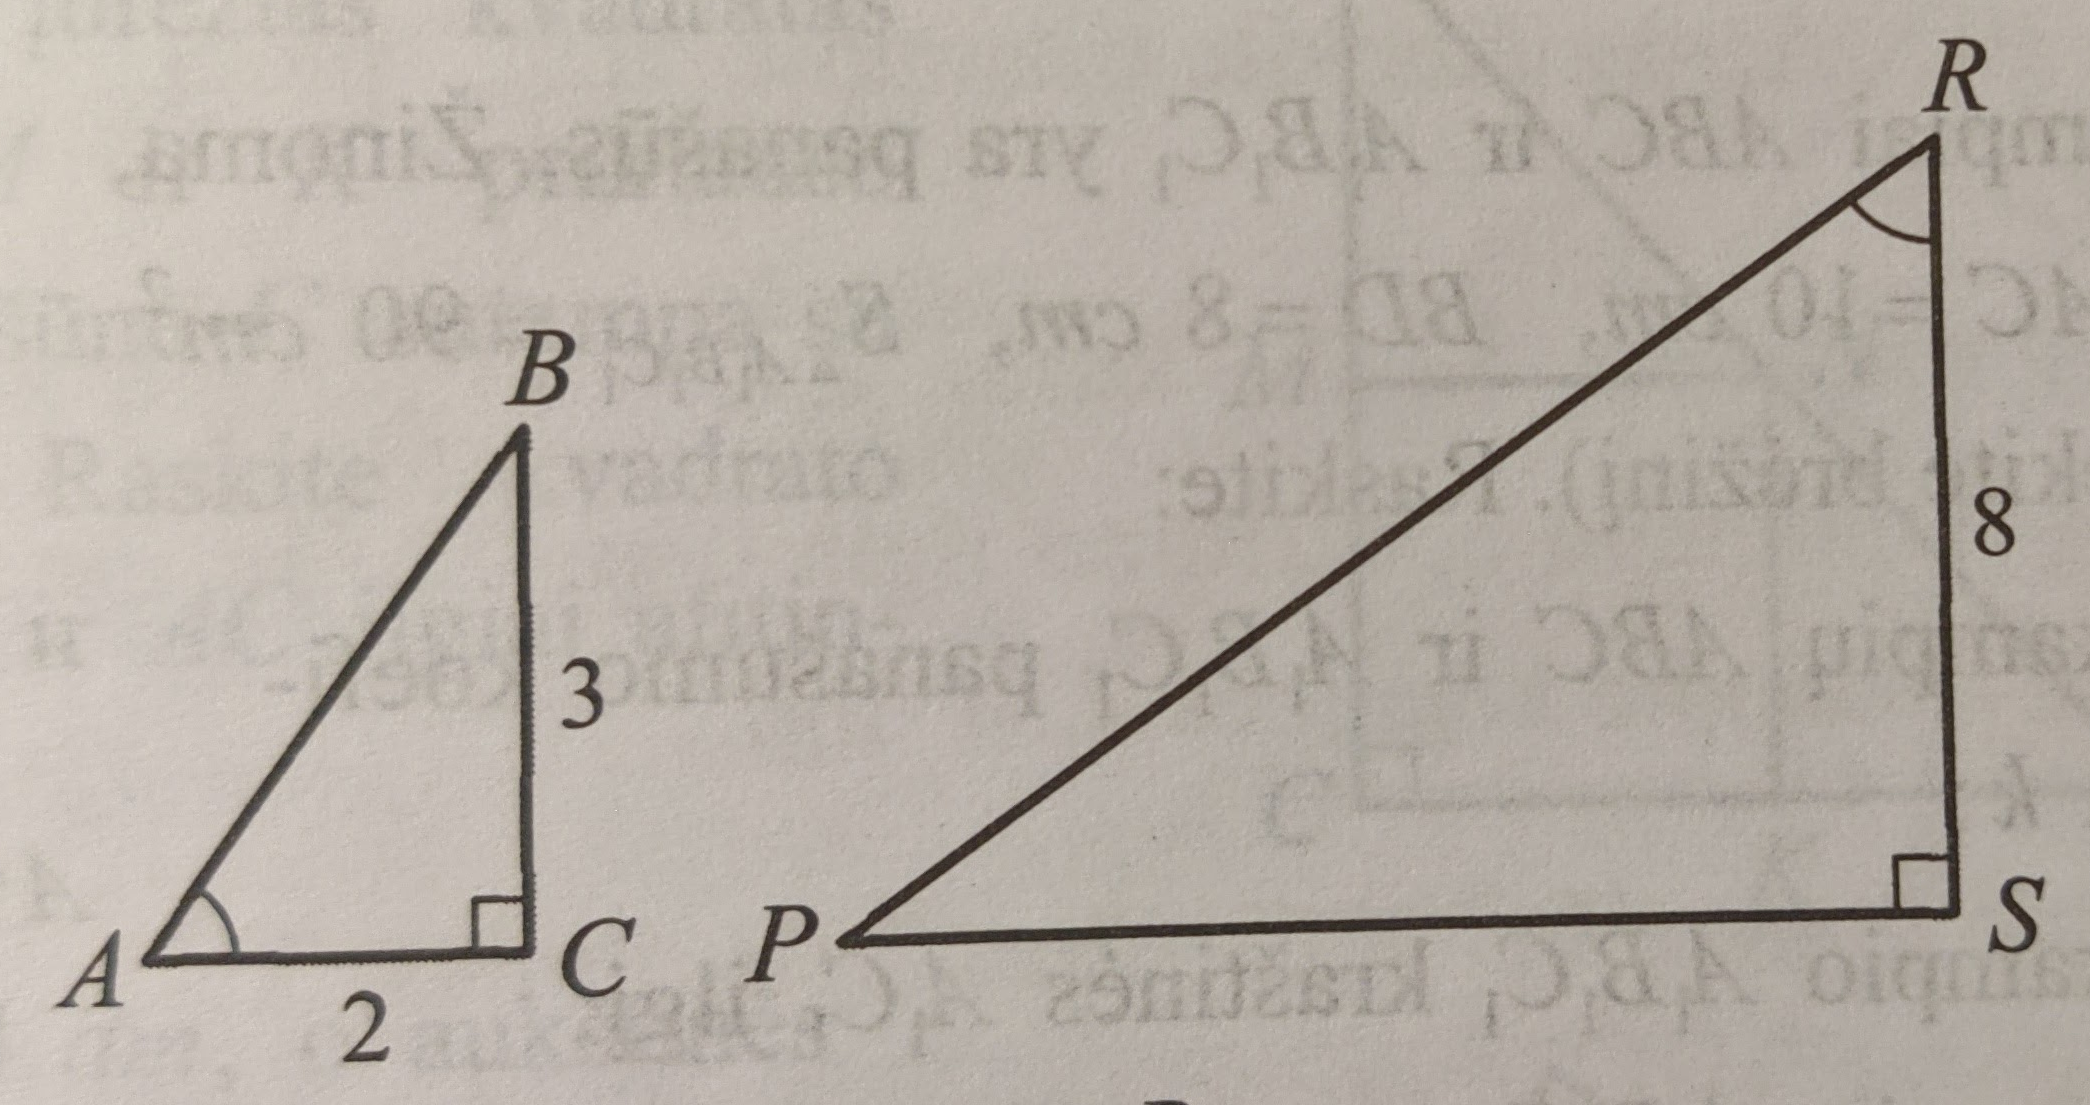
\includegraphics[scale=0.5]{images/triangle_2.png}
      \end{center}
\end{minipage}

\begin{enumerate}
      \setcounter{enumi}{2} % This continues the numbering from the previous enumerate
      \item Trikampiai $ABC$ ir $A_1B_1C_1$ yra panašūs. Žinoma, kad $AB=32 \; cm$,
            $A_1B_1=6,4 \; cm$, $S_{\triangle ABC}=64 \; cm^2$.
            \begin{tasks}[item-format={\normalfont}, after-item-skip=2mm](2)
                  \task Apskaičiuokite trikampio $A_1B_1C_1$ plotą;
                  \task Apskaičiuokite trikampių $A_1B_1C_1$ ir $ABC$ perimetrų santykį.
            \end{tasks}
\end{enumerate}

\subsection*{1 variantas}

\begin{minipage}{0.5\textwidth}
      \begin{enumerate}
            \setcounter{enumi}{0} % This continues the numbering from the previous enumerate
            \item Remdamiesi brėžinyje pateiktais duomenimis:
                  \begin{tasks}[item-format={\normalfont}, after-item-skip=2mm](1)
                        \task Įrodykite, kad trikampiai $ABC$ ir $AED$ panašūs;
                        \task Raskite atkarpos $DE$ ilgį;
                        \task Trikampio $ADE$ plotą.
                  \end{tasks}
      \end{enumerate}

      \begin{center}
            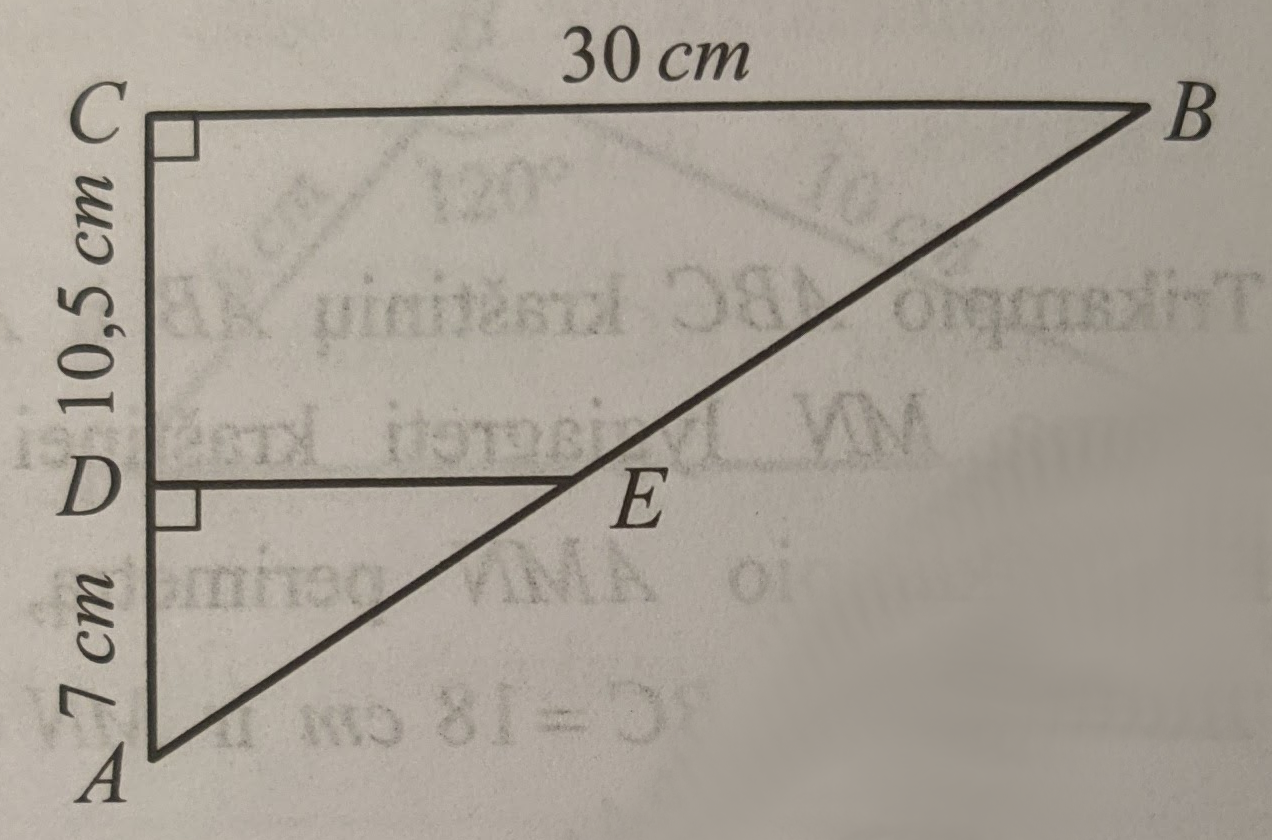
\includegraphics[scale=0.5]{images/triangle_1.png}
      \end{center}

\end{minipage}
\begin{minipage}{0.5\textwidth}
      \begin{enumerate}
            \setcounter{enumi}{1} % This continues the numbering from the previous enumerate
            \item Remdamiesi brėžinyje pateiktais duomenimis, įrodę, kad pateikti trikampiai
                  panašūs, apskaičiuokite trikampio $PRS$ kraštinės $PS$ ilgį.
      \end{enumerate}
      \begin{center}
            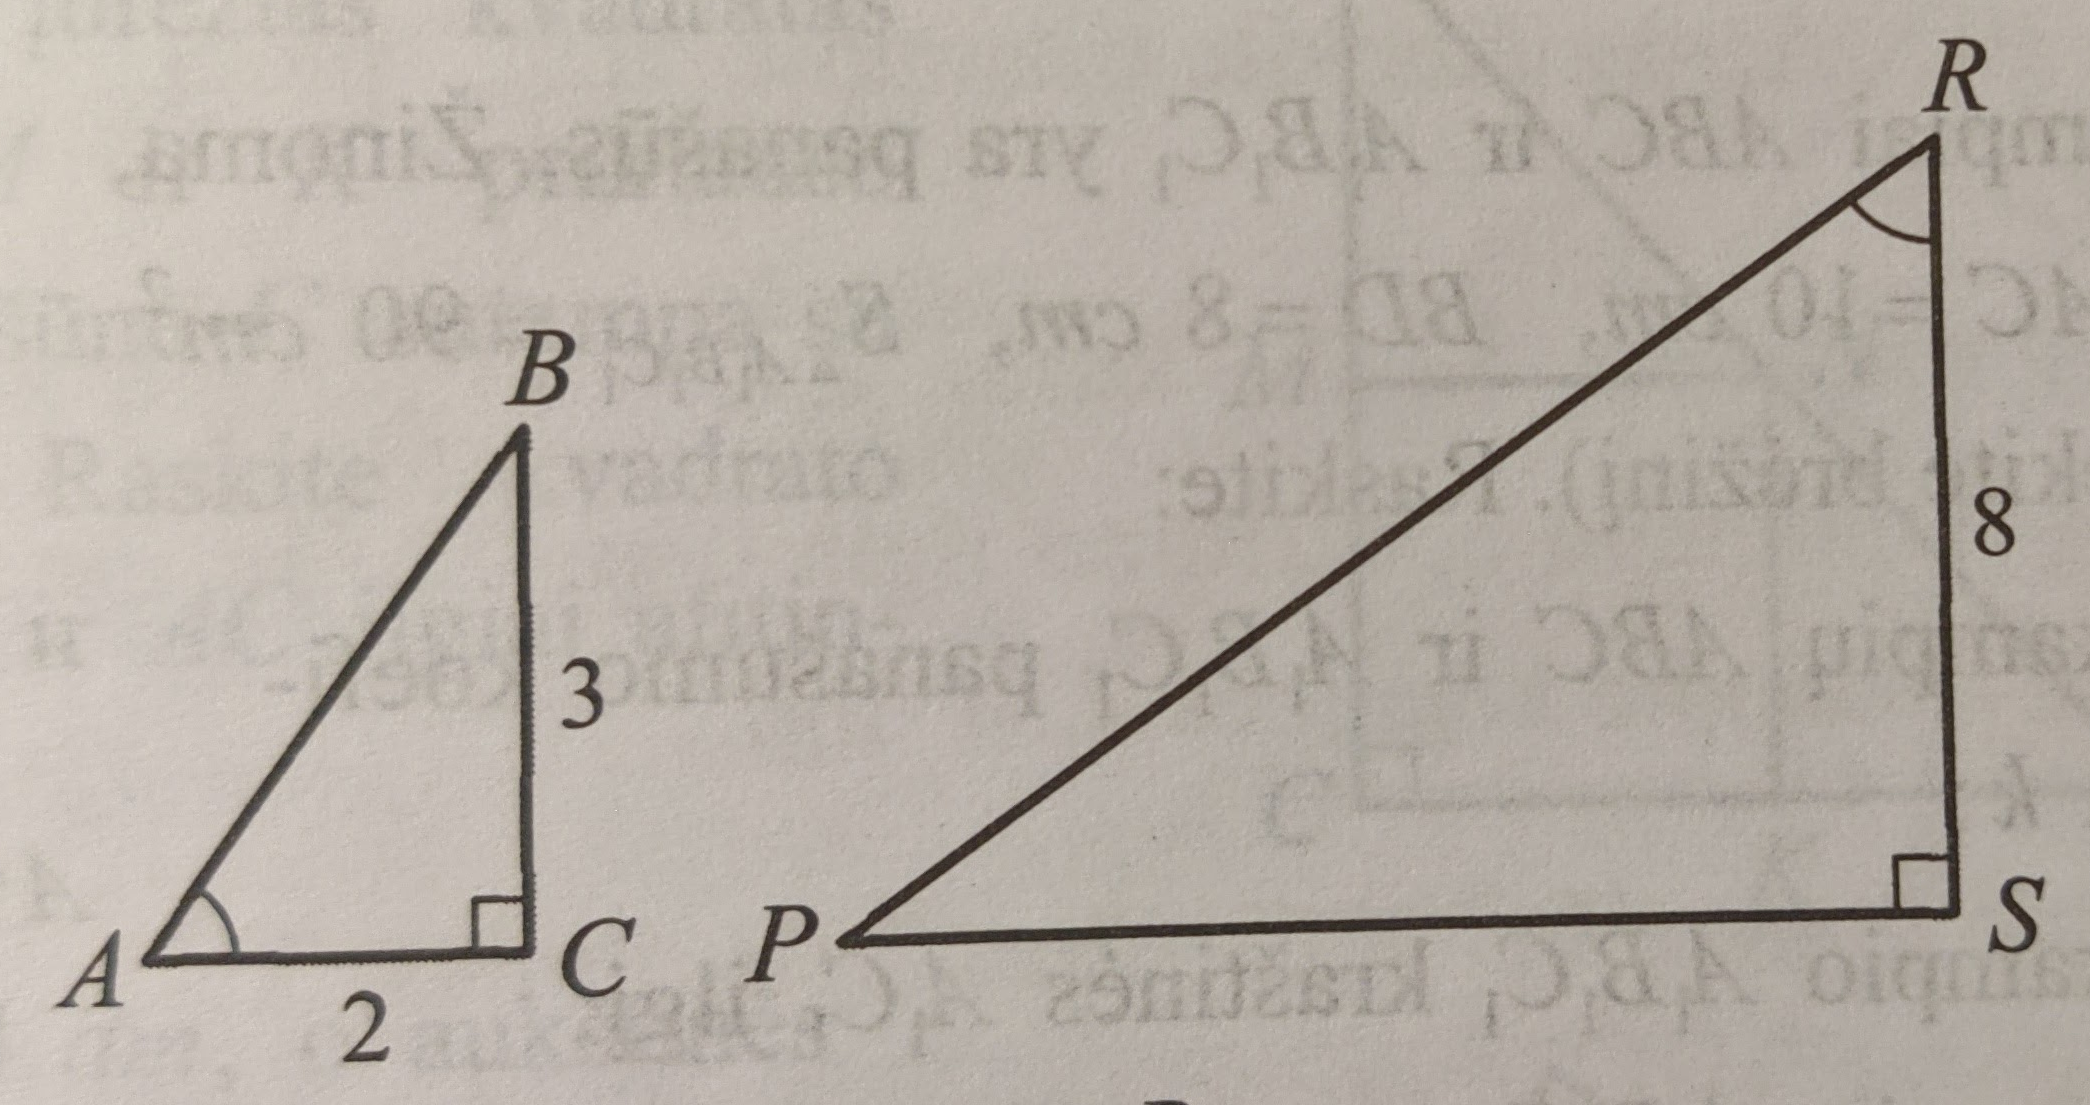
\includegraphics[scale=0.5]{images/triangle_2.png}
      \end{center}
\end{minipage}

\begin{enumerate}
      \setcounter{enumi}{2} % This continues the numbering from the previous enumerate
      \item Trikampiai $ABC$ ir $A_1B_1C_1$ yra panašūs. Žinoma, kad $AB=32 \; cm$,
            $A_1B_1=6,4 \; cm$, $S_{\triangle ABC}=64 \; cm^2$.
            \begin{tasks}[item-format={\normalfont}, after-item-skip=2mm](2)
                  \task Apskaičiuokite trikampio $A_1B_1C_1$ plotą;
                  \task Apskaičiuokite trikampių $A_1B_1C_1$ ir $ABC$ perimetrų santykį.
            \end{tasks}
\end{enumerate}

\end{document}